\documentclass[usenatbib]{mnras}

\usepackage[varg]{newtxmath}
\usepackage{newtxtext}
\usepackage[utf8]{inputenc}
\usepackage{graphicx}
\usepackage{microtype}
\usepackage{xcolor}
\usepackage{fixltx2e}
\usepackage{booktabs}
\usepackage{hyperref}
\usepackage{siunitx}
\usepackage{color}
\hypersetup{colorlinks=True, linkcolor=blue!50!black, citecolor=black,
  urlcolor=blue!50!black}
\usepackage{microtype}

\graphicspath{ {../}, }

\title[Will's extra material]{Extra knot material from Will for the
  Alma paper}

\newcommand\AddressIRyA{Instituto de Radioastronom\'{\i}a y Astrof\'{\i}sica,
  Universidad Nacional Aut\'onoma de M\'exico, Apartado Postal 3-72,
  58090 Morelia, Michoac\'an, M\'exico}

\newcommand\AddressEnsenada{Instituto de Astronom\'{\i}a, Universidad
  Nacional Aut\'onoma de M\'exico, Km 103 Carretera Tijuana-Ensenada,
  22860 Ensenada, Baja California, México}

\author[Fernández-Martín et al.]{
  Alba Fernández-Martín,\textsuperscript{1}
  William J. Henney,\textsuperscript{1}
  M. Teresa García-Díaz,\textsuperscript{2}
  \& S. Jane Arthur\textsuperscript{1}\\
  \textsuperscript{1}\AddressIRyA\\
  \textsuperscript{2}\AddressEnsenada\\
}
\date{Accepted XXX. Received YYY; in original form ZZZ}

\pubyear{2017}
\begin{document}
\label{firstpage}
\pagerange{\pageref{firstpage}--\pageref{lastpage}}
\maketitle

\begin{abstract}
New material written by Will in 2016 December, describing methodology,
results, and interpretation from new knot measurements and fitting.
\end{abstract}

% Select between one and six entries from the list of approved keywords.
% Don't make up new ones.
\begin{keywords}
knots -- knots -- and more knots!
\end{keywords}

\newcommand\nii{\ensuremath{\ion{N}{ii}}}
\newcommand\ha{\ensuremath{\mathrm{H\alpha}}}

\section{Knot classification}
\label{sec:knot-classification}

\begin{figure*}
  \centering
  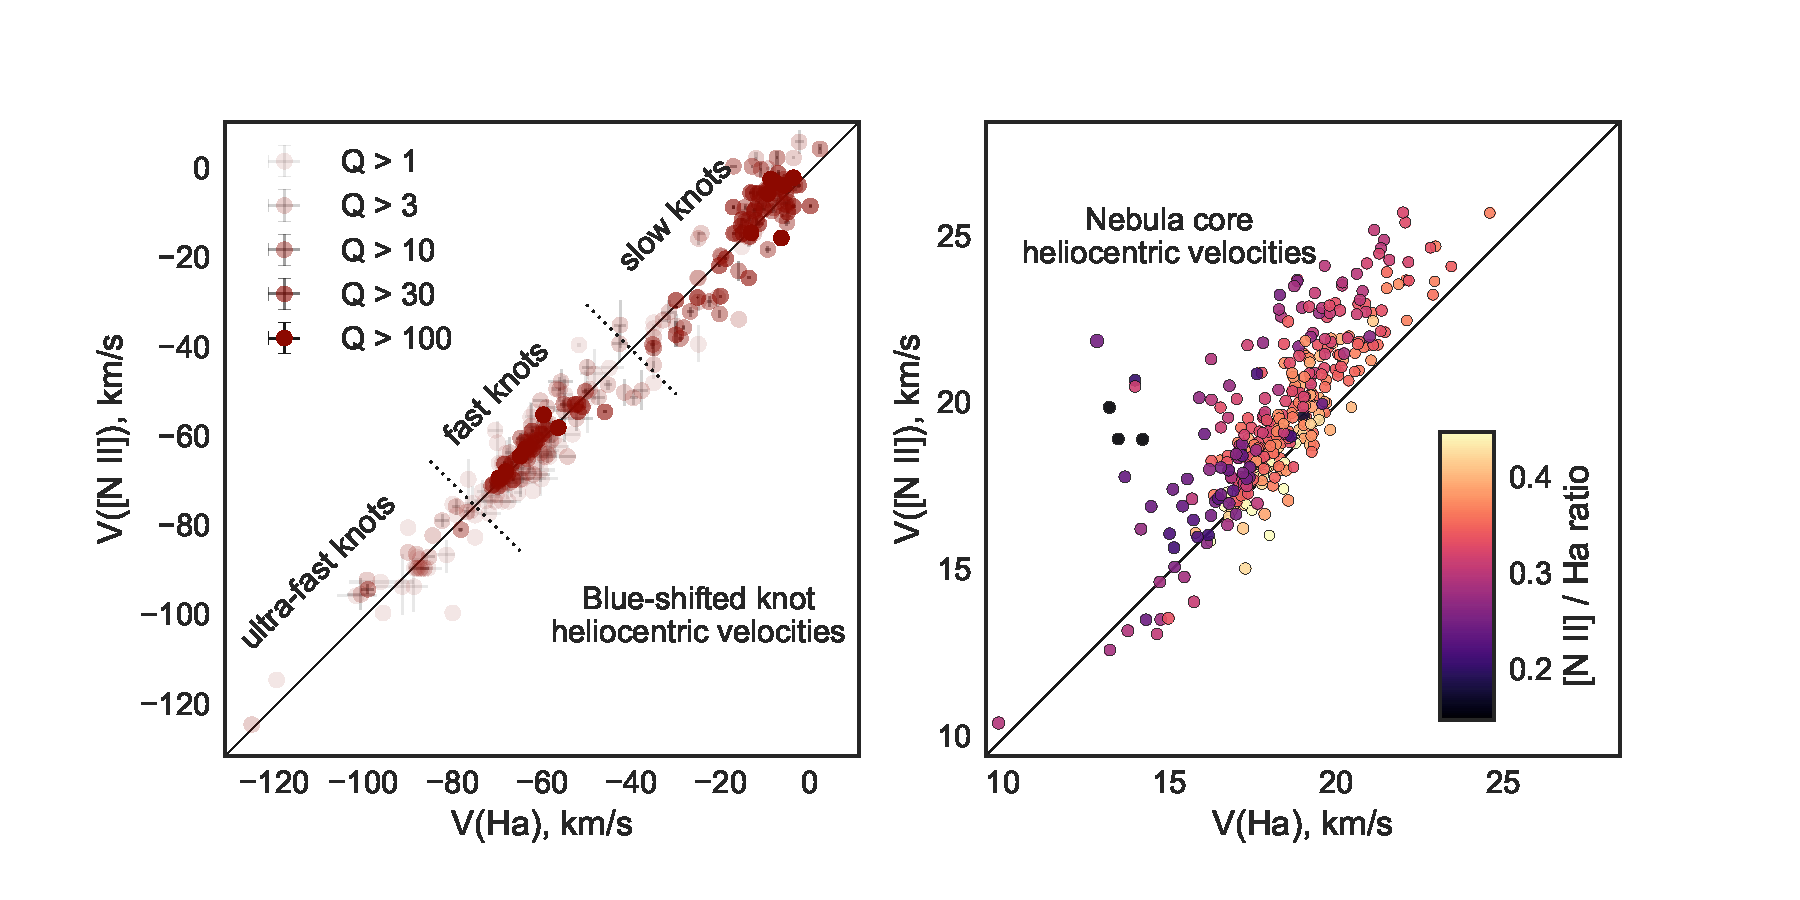
\includegraphics[width=\linewidth]{knot-and-core-velocities-ha-nii}
  \caption{Velocity measurements for the blue-shifted knots (left
    panel) and nebular core (right panel).}
  \label{fig:velocity-ha-nii}
\end{figure*}


\begin{figure}
  \centering
  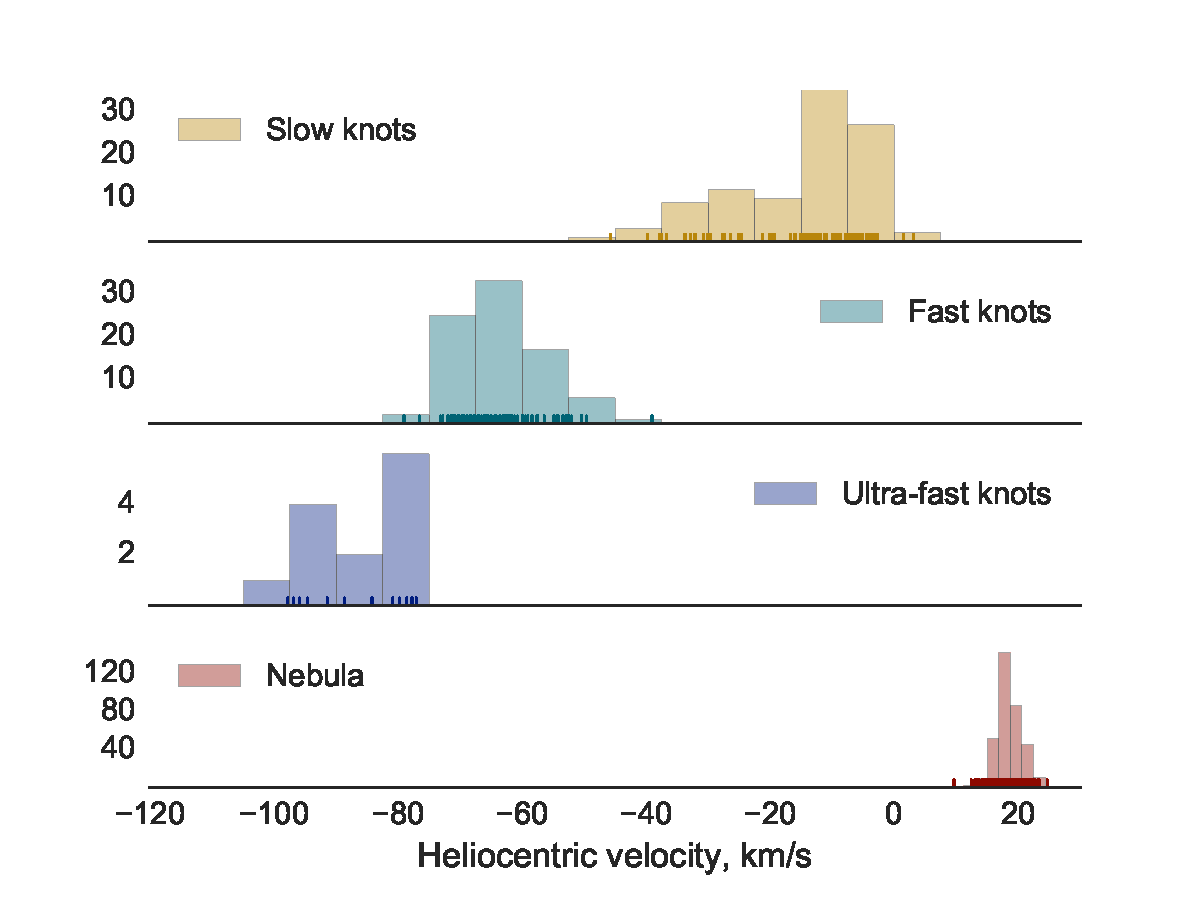
\includegraphics[width=\linewidth]{knot-histogram-vel}
  \caption{Division of knots into three velocity classes.}
  \label{fig:velocity-classes}
\end{figure}

\section{Knot Analysis}
\label{sec:knot-analysis}

\begin{figure}
  \centering
  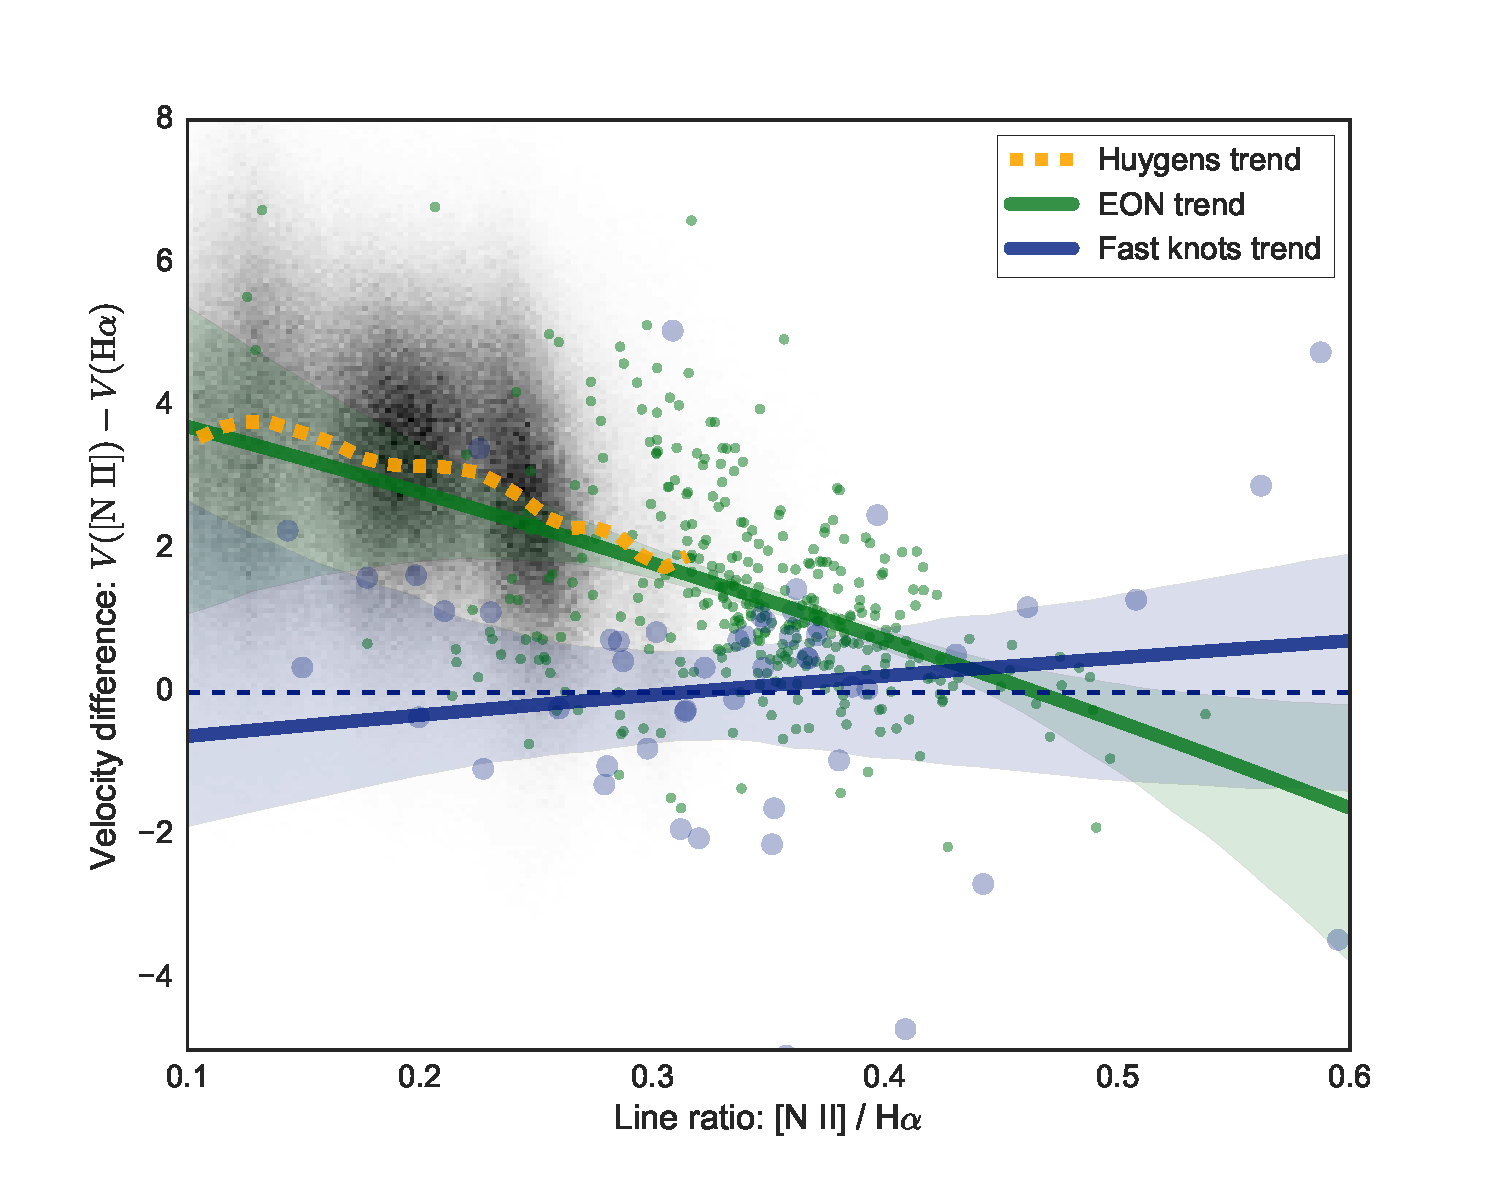
\includegraphics[width=\linewidth]{knot-dv-versus-nii-ha-ratio}
  \caption{Correlation between [\nii]--\ha{} velocity difference,
    \(\Delta V\), versus line ratio, \(R_{[\nii]}\), for different
    datasets. The \textit{grayscale cloud} shows the inner Huygens
    region of the nebula, obtained from
    \(N \approx \SI{2.5e6}{pixels}\) of integral field spectroscopy
    data from the VLT-MUSE instrument \citep{MUSE}, where the
    \textit{orange dashed line} indicates the trend, obtained by
    averaging the \(\Delta V\) values within \(R_{[\nii]}\) bins of
    width 0.01.  \textit{Blue points} show the results for the
    best-measured knots in the ``fast'' velocity class (restricted to
    [\nii] line width \(< \SI{30}{km s^{-1}}\),
    \(N = \SI{68}{knots}\)), while the \textit{blue line} indicates
    the best-fit quadratic trend, with 95\% confidence interval shown
    by the \textit{pale blue band}.  \textit{Green points} show
    results for the low-velocity line core of the western Extended
    Orion Nebula (EON) from sample positions corresponding to all of
    our knot measurements (\(N = \SI{351}{positions}\)), with
    quadratic trend and 95\% confidence interval shown by
    \textit{green line} and \textit{pale green band}, respectively.
    For both datasets from the current study, we have added
    \(\SI{+1}{km s^{-1}}\) to all the [\nii] in order to force an
    average \(\Delta V \approx 0\) for the fast knots.  See text for
    discussion.}
\end{figure}

\bibliographystyle{mnras}
\bibliography{will-alba-refs}

\label{lastpage}
\end{document}

%%% Local Variables:
%%% mode: latex
%%% TeX-master: t
%%% End:
